\documentclass[sigconf,nonacm]{acmart}

\settopmatter{printacmref=false}
\renewcommand\footnotetextcopyrightpermission[1]{}
\pagestyle{plain}

\title{Mining Job Market Data for Career Path Intelligence and Salary Prediction}
\subtitle{CSCI 5502: Data Mining Final Report}

\author{Karthik Alluri}
\affiliation{%
  \institution{University of Colorado Boulder}
  \city{Boulder}
  \state{Colorado}
  \country{USA}}

\author{Shashidhar Reddy Kanaparthi}
\affiliation{%
  \institution{University of Colorado Boulder}
  \city{Boulder}
  \state{Colorado}
  \country{USA}}

\renewcommand{\shortauthors}{Alluri and Kanaparthi}

\begin{abstract}
SkillMap studies skill co-occurrence, job-role structure, and salary tiers in public job-posting data. The cleaned historical cohort contains 34,179 jobs and 436,441 warehouse fact rows. Corrected skill extraction yields 62 general association rules, but clustering remains weak: saved K-Means and DBSCAN silhouettes are 0.0557 and 0.1917. A description-grouped, training-CV-selected fixed XGBoost assessment achieves macro F1 0.695879, one-versus-rest ROC--AUC 0.869863, accuracy 0.700848, and Mid-tier F1 0.569943. These exploratory reused-data results replace test-selected checkpoint scores as the principal controlled assessment. Cached historical-model predictions on 1,149 Adzuna records give macro F1 0.464431; 1,092 salary targets are provider estimates. The Muse confirms one of twenty fixed historical rules under the primary protocol. A bounded improvement sprint rejects employer-text ablation, Mid reweighting, and a low-support technical rule set; a context extractor remains unvalidated. Only a deterministic salary-lineage exporter is integrated, linking all retained jobs without changing salaries or tiers. The study supports descriptive historical patterns and moderate within-cohort prediction, while independent external generalization remains unestablished.
\end{abstract}


\begin{CCSXML}
<ccs2012>
 <concept>
  <concept_id>10002951.10003260</concept_id>
  <concept_desc>Information systems~Data mining</concept_desc>
  <concept_significance>500</concept_significance>
 </concept>
 <concept>
  <concept_id>10010147.10010257</concept_id>
  <concept_desc>Computing methodologies~Machine learning</concept_desc>
  <concept_significance>500</concept_significance>
 </concept>
</ccs2012>
\end{CCSXML}

\ccsdesc[500]{Information systems~Data mining}
\ccsdesc[500]{Computing methodologies~Machine learning}
\keywords{job market analysis, skill mining, association rules, classification, clustering, salary prediction, live validation}

\begin{document}
\maketitle

\section{Introduction}
Online job boards make it easy to search individual openings, but they do not directly show patterns across large collections of postings. A student or job seeker may want to know which skills commonly appear together, whether different job titles share similar skill requirements, or how those patterns relate to compensation. Finding these relationships manually is difficult because the information is distributed across many separate listings.

SkillMap connects skills, role patterns, and salary through a historical mining pipeline and a separate cached-source validation branch. We retain three research questions: (1) which skills consistently appear together and are associated with higher compensation, (2) whether distinct role archetypes emerge beyond traditional job titles, and (3) whether salary tier can be predicted reliably from job-posting features alone. Here, ``associated with'' is descriptive; the data cannot establish a causal return to learning a skill.

\subsection{Completed Contributions}
The completed study provides a common warehouse and skill representation for association mining, classification, clustering, and outlier detection. It documents corrected extraction results, a description-grouped evaluation with training-only model selection, employer-disjoint ablation, and cached cross-source checks. A bounded improvement sprint reports its unsuccessful and unvalidated candidates alongside its successful provenance export. These distinctions matter: a passing integrity check does not imply better prediction, and a different evaluation split does not create an independent test dataset.

\section{Related Work}
The mining methods follow the standard treatment of preprocessing, frequent patterns, classification, and clustering by Han, Pei, and Tong~\cite{han2023}. Khaouja et al.~\cite{khaouja2021} review skill identification from job advertisements, while Senger et al.~\cite{senger2024} organize the terminology, datasets, and deep learning methods used in computational job-market analysis. SkillSpan supplies expert span annotations and guidelines~\cite{skillspan2022}; it motivates independent evaluation of context handling, but its reported neural-model results do not validate SkillMap's regex matcher.

Samwi et al.~\cite{samwi2024} apply Apriori to ICT advertisements, and Debao et al.~\cite{debao2021} use text clustering to examine big-data job requirements. Kablaoui and Salman~\cite{kablaoui2022} study supervised salary prediction. Matbouli and Alghamdi~\cite{matbouli2022} instead predict salaries from occupational and organizational survey features. Their cohorts, targets, and metrics differ from our three-tier posting task, so their scores are not direct baselines.

Three methodological references guide the final audit. H\"am\"al\"ainen and Webb~\cite{hamalainen2019} explain why pattern frequency and lift filters do not control false discoveries across a large search. Kapoor and Narayanan~\cite{kapoor2023} document leakage and evaluation failures in machine-learning-based science, supporting explicit separation of model selection and assessment. Sandve et al.~\cite{sandve2013} advocate recording inputs and computational steps. SkillMap's fixed split manifests and hashed lineage exports address parts of these concerns without claiming complete reproducibility from a clean installation.

\section{Data and Preprocessing}
\subsection{Historical and Cached Sources}
The main historical source contains 123,849 LinkedIn postings from 2023--2024. Its salary-observed, cleaned cohort has 34,179 jobs. A separate LinkedIn jobs-and-skills dataset supplies the vocabulary: its processed table contains 1,294,296 jobs, but these are not additional classifier training records. The data-science salary source is an external descriptive benchmark, not a classification test set. The retained vocabulary has 245 unique skills.

Adzuna and The Muse were fetched on October 14, 2026. They contribute 1,150 and 1,378 cached postings, respectively. Adzuna has 1,149 evaluable cached salary predictions; The Muse has descriptions but no salary targets in the processed snapshot. Neither cache is used for training or model selection. A later fetch date does not isolate a time effect, because source populations, employers, description lengths, and salary-label provenance also differ.

\begin{table}[t]
\caption{Verified saved data objects. Fact rows are not independent jobs.}
\label{tab:data-summary}
\centering\small
\begin{tabular}{p{0.53\columnwidth}p{0.31\columnwidth}}
\toprule
Object & Size \\
\midrule
Raw main-source postings & 123,849 \\
Retained historical jobs & 34,179 \\
Historical warehouse facts & 436,441 \\
Description-grouped assessment & 6,836 jobs \\
Adzuna cached/evaluable & 1,150 / 1,149 \\
Muse cached/eligible for rules & 1,378 / 1,372 \\
Extracted skill vocabulary & 245 \\
\bottomrule
\end{tabular}
\end{table}

\subsection{Salary, Missingness, and Deduplication}
The saved preprocessing excludes 87,776 rows without usable salary, 15 non-USD rows, and 454 implausible salaries. It removes 1,425 exact reposts using company name, title, description, and normalized salary. Such equality is distinct from a suspected template or a shared employer. Later diagnostics find 396 repeated normalized-description groups, containing 472 excess rows, among retained jobs; these are grouping diagnostics, not instructions to delete records.

Existing vendor-normalized annual salary is preserved. The implemented missing-only fallback multiplies the available minimum/maximum midpoint, or median, by 2,080 for hourly, 52 for weekly, 26 for biweekly, 12 for monthly, or 1 for yearly pay. Unknown periods do not imply annual pay. No currency conversion or inferred work-hours adjustment is performed. The saved cohort required zero annualization fills and zero experience-median target imputations; the final investigations do not impute targets. Auditing 36,073 comparable raw salaries found no vendor-versus-formula discrepancy above one cent.

Labels remain Low $\leq\$62,400$, Mid $>\$62,400$ and $\leq\$109,200$, and High $>\$109,200$. These boundaries originated from exact one-third/two-thirds quantiles of the globally processed cohort before splitting. They are frozen task definitions, not training-fold estimates or independently derived labels. Salary and salary-derived predictors are excluded from classification. Missing target exclusion can bias the studied population; title-based family diagnostics do not correct that selection bias.

\subsection{Skill Extraction and Warehouse}
Regex matching includes spelling variants, synonym merging, and nested-phrase handling. A historical six-term correction reduced unrelated senses of driving, organization, supervision, security, reporting, and Excel. Mean detected skills fell from 11.5 to 11.1, and the historical general-rule count fell from 91 to 62. Benefits and development opportunities can still be mistaken for requirements. The later context prototype is not adopted because no independent accuracy labels are available.

SQLite stores one fact row per job--skill relationship, with location, company, time, and industry dimensions. The one-row-per-job view \texttt{v\_jobs} contains 34,179 jobs; salaries must be aggregated through this view rather than over repeated facts. Final read-only checks confirm 436,441 historical facts and exact agreement between the view and retained salary/tier values. Live tables remain separate.

\subsection{Versioned Salary Lineage}
The only integrated sprint improvement is an optional exporter, \texttt{scripts/export\_salary\_lineage.py}. It copies canonical and original source salary strings, records source-file hashes and logical CSV record pointers, and identifies exact raw repost-key groups. All 34,179 retained IDs link to source records. Salary estimate/advertisement status is explicitly unknown for LinkedIn; neither the code nor the paper infers it. Raw group sizes precede filtering and are not deletion counts.

Two full exports were byte-identical, about 2.1 MB compressed each, with zero salary, tier, source-value, pointer, or group-size discrepancies. The exporter changes no dataset, warehouse schema, model, or deduplication rule. Its measurable benefit is auditable regeneration, not increased predictive accuracy.

\section{System Architecture}
Figure~\ref{fig:architecture} retains the original two-branch design. Historical ingestion, cleaning, and warehousing feed the mining tasks. A separate branch applies fixed historical vocabulary, rules, and the historical trained model to cached external postings. The diagram represents the implemented acquisition/validation flow; final validation reuses the caches rather than making API requests. The salary benchmark is descriptive, not classifier training data. The lineage exporter is an optional read-only audit of historical inputs and is not a new training stage.

\begin{figure*}[t]
\centering
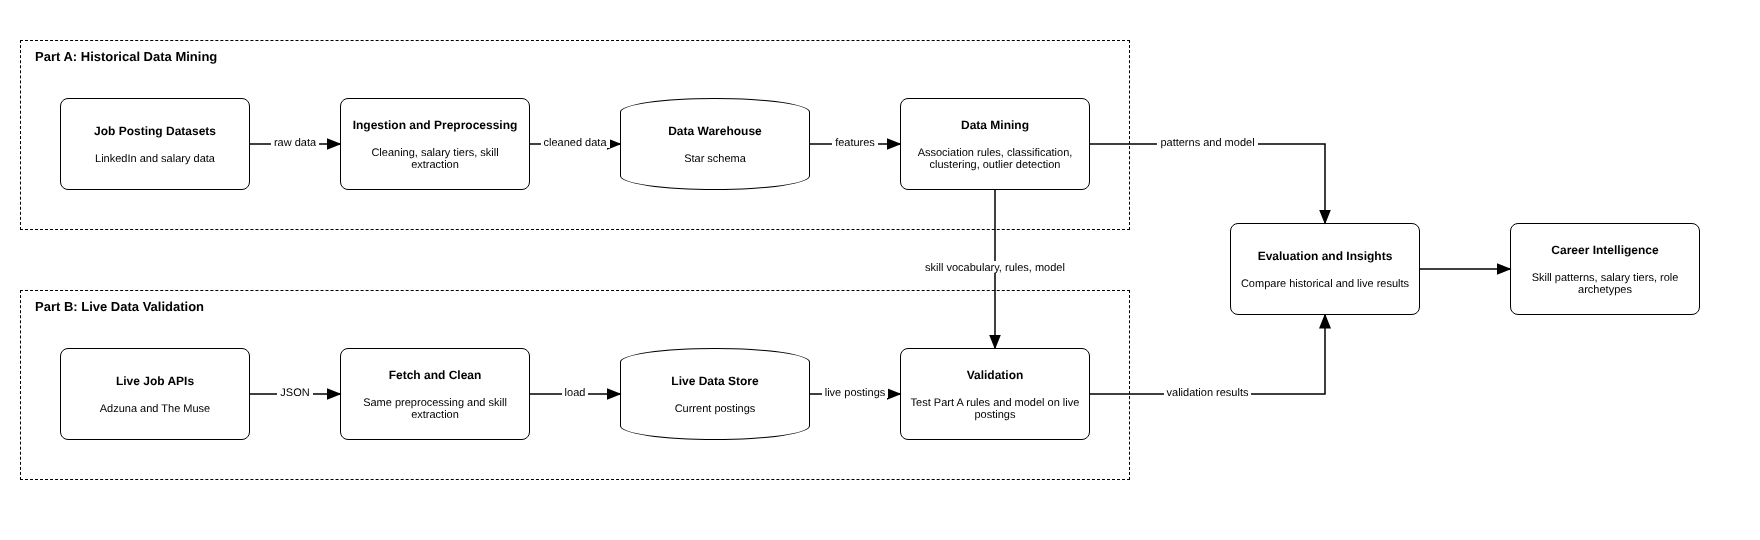
\includegraphics[width=\textwidth]{figures/architecture.png}
\caption{Original pipeline architecture, retained because its historical-mining and external-validation branches remain applicable. API acquisition occurred previously; this final audit uses cached snapshots only. Role archetypes are a research question, not an established output.}
\label{fig:architecture}
\end{figure*}

The React interface reads saved exports. User routes expose exploration, skills, salary, profiles, and cached market data; Admin routes expose model, mining, clustering, quality, and validation evidence. A separately lazy-loaded \texttt{/playground} shell contains prototype views. Its presence in a separate bundle is an implementation fact, not approval to replace production views. Admin navigation is a presentation mode, not demonstrated access control.

\section{Data Mining Methodology}
\subsection{Association Rule Mining}
Each historical job is a transaction. For itemset $X$ and rule $X\rightarrow Y$,
\begin{equation}
\mathrm{support}(X)=\frac{|\{t:X\subseteq t\}|}{N},
\end{equation}
\begin{equation}
\mathrm{confidence}(X\rightarrow Y)=\frac{\mathrm{support}(X\cup Y)}{\mathrm{support}(X)},
\end{equation}
\begin{equation}
\mathrm{lift}(X\rightarrow Y)=\frac{\mathrm{confidence}(X\rightarrow Y)}{\mathrm{support}(Y)}.
\end{equation}
Lift above one denotes positive empirical dependence relative to marginal frequencies, not a significance test or causal effect. Apriori uses support $\geq0.05$, confidence $>0.5$, and lift $>1.5$, before rounding. The denominator includes all jobs, including empty baskets. High-tier mining uses all High jobs as its denominator; reported High shares are then recomputed among all jobs matching the complete itemset. A 0.02-support pass permits rules involving technical skills, which is different from requiring every item to be technical.

\subsection{Classification and Grouped Evaluation}
Base predictors are the 245 skill indicators, experience, company size, top states and industries, and detected-skill count. Text features add at most 50 title terms and 30 company terms. Learned categories, TF--IDF vocabularies, IDF weights, and any scaling are fitted only inside each training fold.

The original stratified 80/20 evaluation compared nominal and ordinal families, but test outcomes influenced family selection. We therefore label its scores historical exploratory results. The documented corrected comparison uses five-fold stratified description grouping (seed 2026), selects outer fold zero, and performs three-fold grouped training CV (seed 2027). Normalized descriptions are HTML-unescaped, tag-stripped, lowercased, and whitespace-normalized; missing descriptions receive distinct singleton keys. It compares fixed nominal logistic, ordinal Logistic IT, and XGBoost candidates using training CV only. Fixed XGBoost uses 200 trees, depth four, learning rate 0.1, subsample one, and one CPU thread. Its saved fold-zero probabilities independently reproduce the corrected checkpoint metrics during this final audit; no model is fitted in this phase.

For each class, $F1=2PR/(P+R)$; macro F1 averages Low, Mid, and High equally. ROC--AUC averages one-versus-rest class ranking performance. The original targets remain macro F1 $>0.75$ and AUC $>0.80$. This regrouping eliminates normalized-description overlap, but it cannot undo prior inspection of these data, historical global tier construction, or unresolved near duplicates. It is a corrected exploratory assessment, not an untouched final test or evidence that grouping alone caused a score change.

\subsection{Clustering and Outlier Detection}
K-Means and DBSCAN operate on multi-hot detected skills. The saved K-Means sweep selects $k=3$; the saved DBSCAN sweep selects $\epsilon\approx2.83$, \texttt{min\_samples}=20, requiring at least two clusters and at most 50\% noise. Silhouette is
\begin{equation}
s=\frac{b-a}{\max(a,b)},
\end{equation}
where $a$ is within-cluster distance and $b$ is distance to the nearest alternative cluster. Saved silhouette estimates use a fixed 10,000-job sample, excluding DBSCAN noise. PCA and t-SNE visualize structure; visual islands are not independent cluster validation.

Isolation Forest uses skill indicators, experience, and salary, with 300 trees, contamination 0.01, and seed 42. Its fixed contamination determines the approximate flagged count. Salary mismatch is a separate descriptive diagnostic within cluster/experience groups, not an externally labeled anomaly target.

\subsection{Cached External Validation}
The Adzuna analysis scores 1,149 fixed historical predictions; it does not evaluate the newer grouped experimental fit. The cache lacks class probabilities, so external ROC--AUC is unavailable. Salary targets include provider estimates and cannot be treated as verified compensation. The historical training-majority baseline is Low. Always-High is an evaluation-label majority oracle and is explicitly not a training-selected baseline.

Muse validation fixes the historical top 20 rules, requires at least two detected skills per posting, and applies the same primary thresholds. A company cap retains at most 25 postings per employer before eligibility filtering. A separately declared 0.02-support sensitivity is not chosen using confirmation counts. Employer-cluster bootstrap intervals use 200 replicates and seed 42; they condition on the fixed cached predictions/rules and omit model-fitting uncertainty.

\subsection{Controlled Improvement Experiments}
The bounded sprint froze seeds, observations, criteria, and candidate scope before outcomes. Employer--description connected components produce 10,677 groups, largest 345 jobs. Five identical component folds compare fixed XGBoost with versus without company TF--IDF; acceptance requires mean paired macro-F1 gain $\geq0.01$ and no class-F1 loss $>0.02$. Employer identity uses source IDs and normalized names; unresolved aliases and unknown identities remain limitations.

Mid-class multipliers are limited to 1.00, 1.15, and 1.30. Within each of five description-grouped outer folds, three inner folds select by mean training-validation macro F1, with ties preferring the smaller multiplier. Outer-fold predictions assess the selected rule separately. Acceptance requires Mid-F1 gain $\geq0.03$, no macro decline, Low/High losses $\leq0.01$, and extreme-class error increase $\leq0.005$.

The technical-pair experiment fixes ten candidates, support in $[0.001,0.02)$, at least ten pair employers and twenty employers for each member, lift $\geq1.5$, and at least one directional confidence $>0.5$. Component fold zero is validation; the rest is discovery. It applies Holm correction over the fixed family and 500 whole-component bootstrap replicates with simultaneous lift lower bounds. Validation precision must reach 80\%, with accepted lower bounds above one. Row-level Fisher tests assume independent records, so employer dependence limits their interpretation; the component bootstrap provides a separate dependence-aware check. Only discovery-selected pairs enter the precision denominator.

A separate occurrence-level context prototype distinguishes employer offers, responsibilities, mixed contexts, and unresolved mentions. It preserves original matches and offsets and supplies a review rubric and 48 examples. No human labels are invented. Its prespecified accuracy gate---50\% fewer benefit false positives with at most two percentage points recall loss---cannot be tested without independent annotation.

\section{Results}
\subsection{Historical Association Patterns}
The corrected historical extraction produces 284 frequent itemsets and 62 general rules passing all filters. The saved general CSV contains the top 20, not all 62. PowerPoint $\rightarrow$ Excel has lift 6.1084, support 0.0577, and confidence 0.9150. Among 810 jobs matching Python and engineering, 81.48\% are High tier; the overall High share is 33.26\%. These describe the selected historical population, not causal pay premiums.

\begin{figure*}[t]
\centering
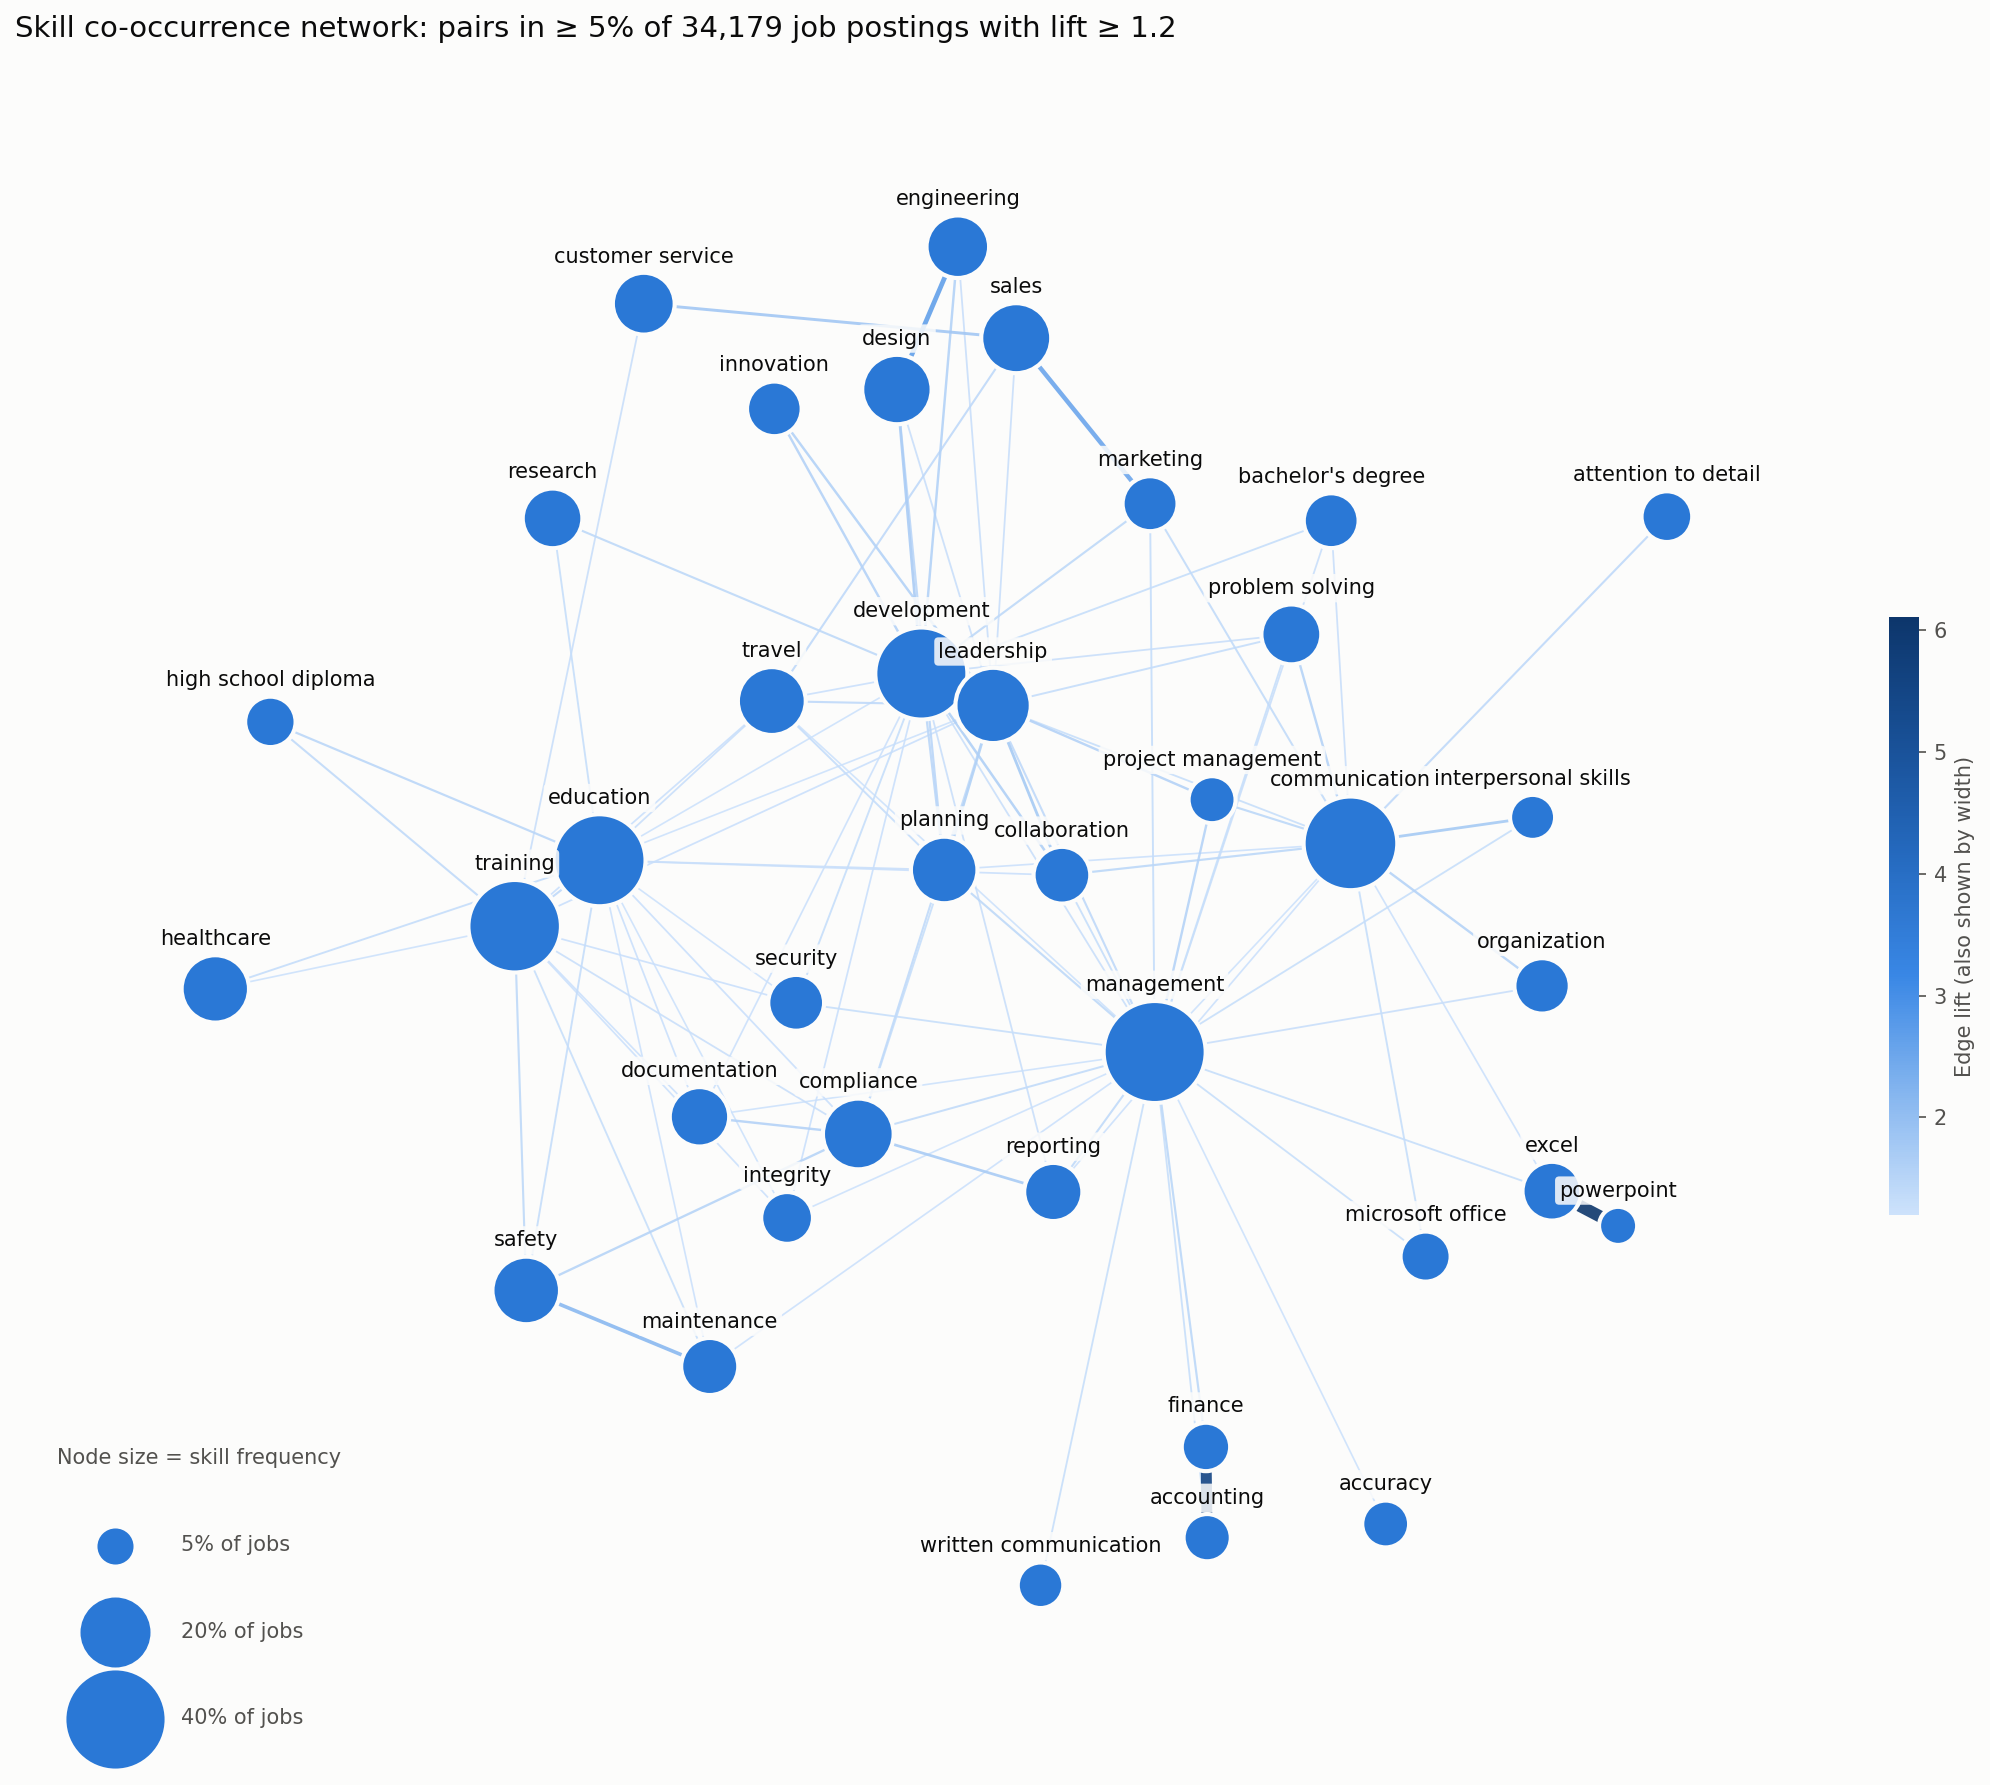
\includegraphics[width=0.78\textwidth]{figures/skill_network_verified.png}
\caption{Saved post-extraction historical skill network, sourced from \texttt{outputs/04\_skill\_network.png}. Pairs meet 5\% support; displayed edges additionally have lift at least 1.2. Node area shows prevalence and edge width/color show lift. This display threshold differs from the rule filter.}
\label{fig:skillnetwork}
\end{figure*}

The technical-involvement pass yields ten rules, but these mix technical and general skills. Requiring all items to be technical yields no rule at 2\% support. Python--SQL appears in 524 jobs (1.53\%), illustrating the support restriction. Lowering support alone is not evidence of better mining quality; the separately controlled pair investigation addresses replication.

\subsection{Corrected Classification and Checkpoint Reconciliation}
Table~\ref{tab:classification} separates evaluations that the checkpoint text previously conflated. The corrected fold-zero assessment uses 27,343 training and 6,836 assessment jobs, with no normalized-description overlap. Macro F1 is 0.695879, AUC 0.869863, and accuracy 0.700848. Low/Mid/High F1 values are 0.779258, 0.569943, and 0.738435. Ranking exceeds the preset AUC target, but macro F1 misses its target. Figure~\ref{fig:confusion} shows the remaining Mid-class ambiguity: 524 Mid jobs are predicted Low and 526 High.

\begin{table*}[t]
\caption{Classification evidence by protocol. Checkpoint values are approximate claims in the preserved original text; later historical values come from saved CSVs. The rows do not estimate a paired improvement or regression.}
\label{tab:classification}
\centering\small
\begin{tabular}{p{0.27\textwidth}p{0.27\textwidth}rrr}
\toprule
Evidence & Assessment protocol & Macro F1 & AUC & Accuracy \\
\midrule
Original checkpoint, pre-fix & Stratified split; test-influenced selection & $\sim0.728$ & $\sim0.891$ & $\sim0.729$ \\
Post-extraction historical CSV & Historical stratified split; exploratory & 0.7273 & 0.8921 & 0.7285 \\
Corrected fixed XGBoost & Description-grouped fold 0; training CV selection & 0.695879 & 0.869863 & 0.700848 \\
\bottomrule
\end{tabular}
\end{table*}

The older tuned text model used a different configuration and split. Extraction changes, model scope, grouping, and selection rules all differ, so subtracting the rows would not isolate leakage or an extraction effect. The original historical model remains the canonical saved model; the corrected experimental fit was not promoted. The original feature-importance figure is preserved as an asset but is not presented as an explanation of the corrected classifier.

\begin{figure}[t]
\centering
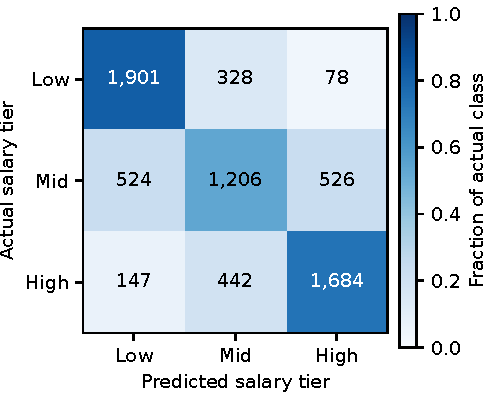
\includegraphics[width=\columnwidth]{figures/grouped_confusion.pdf}
\caption{Corrected description-grouped fold-zero predictions on 6,836 jobs. Cells show counts; color is recall normalized within each actual class. The figure is reconstructed from saved Phase 2 probabilities/predictions, not a newly fitted model.}
\label{fig:confusion}
\end{figure}

\subsection{Clustering and Outliers}
The post-extraction historical K-Means silhouette is 0.0557 and Davies--Bouldin index 4.7527. DBSCAN reaches silhouette 0.1917 and Davies--Bouldin 0.9226, with 29.13\% overall noise. Both miss silhouette $>0.50$; DBSCAN meets Davies--Bouldin $<1$. Its largest cluster contains about 99.9\% of assigned, non-noise jobs, so a nominal two-cluster solution provides weak evidence for useful archetypes. Of 34,179 jobs, 268 have no matched skills and are excluded from these cluster fits.

\begin{figure*}[t]
\centering
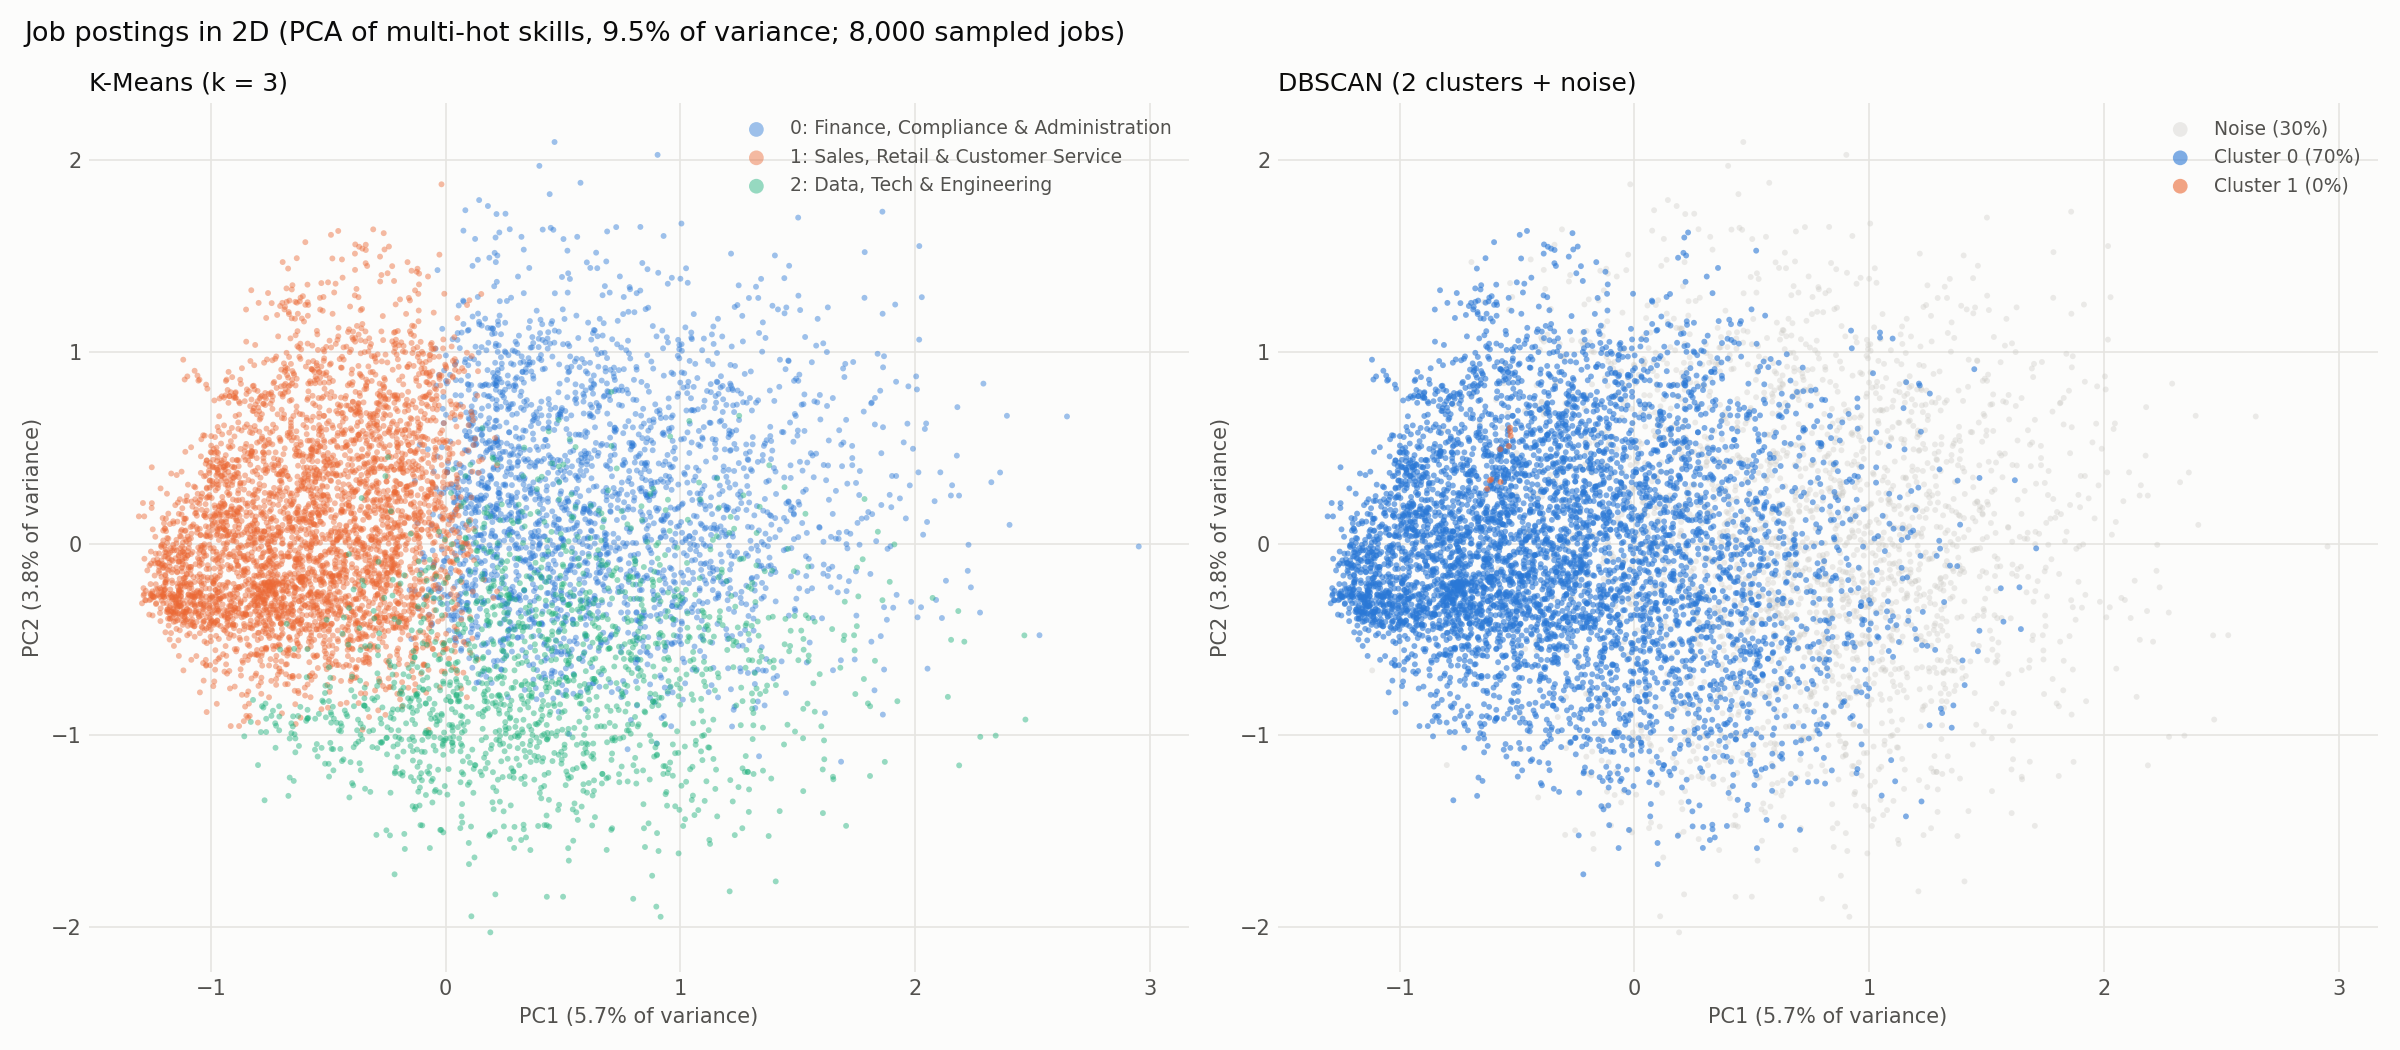
\includegraphics[width=\textwidth]{figures/cluster_pca_verified.png}
\caption{Saved post-extraction PCA visualization of 8,000 sampled jobs, sourced from \texttt{outputs/06\_clusters\_pca.png}. The two dimensions explain 9.5\% of variance. Displayed sample noise is rounded and differs from the full-cohort DBSCAN noise fraction; separation must be assessed in the original feature space.}
\label{fig:pca}
\end{figure*}

The groups support broad descriptive summaries, including a Data, Tech \& Engineering profile, but their weak separation does not establish natural role classes. Isolation Forest flags 342 jobs as dictated by 1\% contamination. Flagged jobs average 30.1 detected skills versus 11.1 overall; anomaly score correlates 0.954 with skill count. Salary mismatches occur in 5.8\% of flagged jobs versus 4.6\% overall. Thus the detector primarily identifies skill-dense descriptions, not verified salary errors.

\subsection{Cached-Source Transfer}
Table~\ref{tab:live} reports recalculated cached Adzuna performance. On 1,149 records from 660 employers, accuracy is 0.579634 and macro F1 is 0.464431. Employer-bootstrap 95\% intervals are [0.540444, 0.612650] for accuracy and [0.424557, 0.495394] for macro F1. Estimated-salary records number 1,092; only 57 are advertised. Their respective accuracies are 0.585165 and 0.473684. The advertised subset is too small and selected to establish general external accuracy.

\begin{table}[t]
\caption{Cached Adzuna comparisons on the same 1,149 records. Always-High is a descriptive evaluation-label oracle.}
\label{tab:live}
\centering\small
\begin{tabular}{p{0.48\columnwidth}rr}
\toprule
Predictor & Accuracy & Macro F1 \\
\midrule
Historical saved classifier & 0.579634 & 0.464431 \\
Training-majority Low & 0.067015 & 0.041871 \\
Always-High oracle & 0.620540 & 0.255281 \\
\bottomrule
\end{tabular}
\end{table}

The classifier has lower accuracy than the High oracle but higher macro F1. Short Adzuna snippets and estimated labels limit comparability with full historical descriptions. These are cached predictions of the historical model, so they do not directly test the corrected grouped model.

Muse confirms one of twenty fixed rules on 1,372 eligible postings: PowerPoint $\rightarrow$ Excel. After capping employers at 25, 602 of 606 postings are eligible and a different rule, marketing $\rightarrow$ sales, confirms (also 1/20). The predeclared lower-support sensitivity confirms 3/20 and 4/20, respectively; it does not replace the primary threshold. The checkpoint's 2/20 predates the extraction correction. Neither one dated source comparison nor source-specific skill prevalence establishes a temporal market trend.

\subsection{Final Controlled Sprint}
Table~\ref{tab:sprint} summarizes all five investigations using their fixed acceptance criteria. ``PASS'' for provenance means a verified integrity/reproducibility deliverable, not a salary-accuracy gain. Paired uncertainty uses 500 fixed-prediction group bootstrap replicates (seed 2028); it omits refitting and model-selection uncertainty.

\begin{table*}[t]
\caption{Final sprint outcomes. Model metrics are pooled across five outer folds unless explicitly called mean-fold gains. Only the provenance exporter and its tests were integrated.}
\label{tab:sprint}
\centering\small
\begin{tabular}{p{0.14\textwidth}p{0.24\textwidth}p{0.35\textwidth}p{0.14\textwidth}}
\toprule
Investigation & Baseline $\rightarrow$ candidate & Fixed-gate finding & Outcome \\
\midrule
Salary lineage & No versioned sidecar $\rightarrow$ 34,179 source-linked rows & 100\% links; zero salary/tier changes; byte-identical exports & PASS \\
Employer text ablation & Macro F1 0.676782 $\rightarrow$ 0.676865 & Mean-fold gain 0.000050 $<0.01$; pooled-gain CI [$-0.002141$, 0.002403] & FAIL \\
Context extraction & Frozen matches $\rightarrow$ occurrence prototype & 81,635 preserved spans; zero independent labels; accuracy unknown & UNVALIDATED \\
Mid adjustment & Mid F1 0.564960 $\rightarrow$ 0.594831 & Gain 0.029872 $<0.03$; High loss 0.013358 $>0.01$ & FAIL \\
Technical pairs & No validated low-support list $\rightarrow$ fixed-family check & 3/4 discovery-selected pairs confirm: 75\% $<80\%$ & FAIL \\
\bottomrule
\end{tabular}
\end{table*}

Employer-fold macro-F1 standard deviations are 0.01029 with company text and 0.01105 without it. The ablation does not support an accuracy benefit from removing company terms. Its employer-disjoint scores are not compared with description-grouped fold zero as evidence of improvement or regression.

Nested Mid adjustment raises macro F1 from 0.689341 to 0.693257 and reduces extreme-class errors from 3.578\% to 2.902\%. Nevertheless, Mid gain misses 0.03 without rounding up, and High F1 violates the loss guardrail. Its Mid-gain interval is [0.025659, 0.034131]; the guardrail failure still rejects integration. The context candidate remains unvalidated even though its offsets and preservation tests pass.

Docker--Kubernetes, Spark--Python, and Tableau--SQL meet the pair validation checks, with simultaneous lift lower bounds 51.84, 13.58, and 12.45. JavaScript--TypeScript fails validation confidence (0.4615 in its stronger direction), leaving precision at 75\%. Dropping this failure after seeing validation would change the fixed candidate question; the rule-set candidate is therefore rejected. The bootstrap's simultaneous-tail estimates have limited resolution at 500 replicates, and sparse-pair lift can be large because marginal prevalence is small.

\section{Answers to the Research Questions}
\subsection{Q1: Which skills consistently appear together and are associated with higher compensation?}
Historical data supports interpretable combinations such as finance/accounting and Python/engineering. Python/engineering jobs are disproportionately High tier, but the study does not estimate causal skill premiums or control all occupational confounding. Only 1/20 fixed general rules confirms on the primary Muse check, and the controlled low-support technical candidate misses its replication gate. The answer is therefore positive for within-source descriptive relationships, with limited demonstrated cross-source stability.

\subsection{Q2: Do distinct role archetypes emerge beyond titles?}
The tested multi-hot representations and algorithms show weak separation. Broad profiles are useful summaries, but silhouette values remain below target, DBSCAN assigns almost all non-noise records to one cluster, and outliers mostly reflect skill count. These negative results concern the tested methods; they do not prove that all representations or role taxonomies must fail.

\subsection{Q3: Can salary tier be predicted reliably from posting features alone?}
The corrected grouped model has useful ranking performance (AUC 0.869863), but macro F1 0.695879 misses the original target and Mid F1 remains 0.569943. Employer-disjoint evaluation and cached historical-model transfer add limitations rather than evidence of deployment reliability. Salary-tier prediction is moderately informative within the studied cohort; reliable employer-independent and external performance remains unestablished.

\section{Discussion and Limitations}
\subsection{Evaluation and Generalization}
The strongest methodological correction is separating selection from assessment and keeping preprocessing fold-contained. It does not erase the original test-influenced model selection. These are reused development data, and globally derived labels, unresolved templates, company aliases, and missing employer IDs remain threats. Changing the grouping question also changes the generalization target: description-disjoint and employer-disjoint scores must be interpreted separately.

External validation is particularly constrained. Cached Adzuna labels are mostly estimates, not independently verified salaries, and the advertised subset has only 57 jobs. The Muse has no salary target and validates a fixed descriptive rule set rather than the classifier. Different sources and description lengths confound chronological interpretation. We cannot claim independent final validation, temporal demand trends, or causal effects of skills.

\subsection{Extraction, Structure, and Negative Results}
Context matters when a posting offers training rather than requiring delivery of training. Narrow historical sense corrections reduce known noise, but the new context prototype has no independent accuracy labels and is excluded. Neither more extracted skills nor more mined rules is automatically better. Weak clustering and skill-count-driven outliers similarly restrict the interpretations supported by unsupervised outputs.

The sprint's negative results are substantive: company-text removal has no required gain; Mid reweighting trades away too much High-tier performance; the technical rule set falls below its fixed replication threshold; and context accuracy is unknown. The provenance exporter is accepted because it adds a reproducible audit path while preserving all numerical targets and inputs. It supplies no evidence that prediction became more accurate.

\section{Future Work}
The next useful extraction study requires independently adjudicated, employer-separated span labels, including implicit and term-absent positives. A genuinely new salary evaluation requires an explicit source/overlap design and separation of advertised and estimated compensation; simply training on cached snapshots would not satisfy this need. Employer alias resolution and reviewed near-duplicate templates could strengthen grouping. Alternative role representations need resampling and employer-stability evaluation rather than selection for attractive two-dimensional plots. Dependency locking, actual Python 3.12 clean-environment execution, and rendered paper/browser acceptance remain reproducibility tasks. No second snapshot or new model is claimed here.

\section{Reproducibility}
\subsection{Artifacts, Seeds, and Commands}
Historical source modules, numbered notebooks, saved CSVs, SQLite, and model files remain unchanged. Some notebook outputs predate the extraction correction; the saved module summaries and explicit artifact provenance take precedence. The controlled evaluation uses outer seed 2026, inner seed 2027, and one numerical thread. Cached validation uses seed 42; sprint paired bootstraps use seed 2028. The original 245-skill vocabulary and salary cutoffs remain frozen.

The retained Phase 2 directory, \texttt{/private/tmp/skillmap-evidence-v1-20261115/}, contains protocol, split manifests, prediction arrays, per-investigation results, and SHA-256 inventories. It is local temporary evidence, not a durable published archive; the repository alone does not reproduce all sprint results. The report's confusion-matrix source and plotting script preserve the small numerical figure input independently. Full archival packaging of experimental predictions remains unfinished.

The following commands use fresh external destinations and do not fit models or request job data:
\begin{verbatim}
python -B -m scripts.export_salary_lineage \
  --root . --out-dir /tmp/new-lineage-v1
python -B -m scripts.validate_cached_live \
  --root . --out /tmp/new-cache-audit
python -B -m scripts.check_offline_environment \
  --root . --out-dir /tmp/new-env-audit --pytest
\end{verbatim}
Use the installed virtual-environment interpreter and set numerical thread counts to one. The environment checker isolates Python caches and test fixtures externally and verifies a socket/DNS guard. Do not run historical pipeline entry points against canonical paths for a validation-only task: some rebuild the database or overwrite artifacts.

\subsection{Final Validation and Remaining Checks}
The final installed-environment audit passes 154 backend tests, with six undefined-precision warnings from synthetic classifier fixtures, and passes installed requirement constraints and \texttt{pip check}. Frontend checking passes TypeScript and all 110 tests. A production build to a fresh external destination succeeds, retaining a separate lazy playground bundle; Vite warns about the large main bundle. Route, navigation, and chart tests execute in jsdom. They are not a real-browser visual or responsive acceptance test.

The earlier Phase 2 suite had 57 passing tests, and provenance integration had 33 targeted passing tests; these are different scopes, not accuracy measurements. Final SHA-256 checks protect original sources, report assets, datasets, models, saved metrics, and frontend files. Requirements specify lower bounds rather than a lockfile. Passing in the installed Python 3.14 environment does not establish clean-install reproducibility or execution of the declared Python 3.12 CI target.

No LaTeX engine is available in the checked environment and the checkpoint PDF was not supplied locally. The original ACM class, authors, and formatting directives are preserved, and figure/citation paths are checked statically. Compilation, page-level visual comparison, overfull-box detection, and final bibliography rendering remain unverified. No alternative PDF template is substituted for the original source.

\section{Conclusion}
SkillMap provides a completed historical mining pipeline with explicit limits on its findings. Sixty-two filtered association rules summarize within-source co-occurrence, while weak clustering and limited cached-source confirmation constrain role and transfer claims. Corrected description-grouped assessment yields macro F1 0.695879 and AUC 0.869863, with substantial Mid-tier errors and no independently established deployment accuracy. Controlled improvement experiments reject or defer all predictive/extraction/mining candidates. The accepted lineage exporter adds verifiable source mapping for all 34,179 jobs without changing salaries, tiers, or model outcomes. These measured boundaries are the final research findings rather than milestones to be replaced by unsupported improvements.

\begin{thebibliography}{11}
\bibitem{han2023}
Jiawei Han, Jian Pei, and Hanghang Tong. 2023. \textit{Data Mining: Concepts and Techniques}, 4th ed. Morgan Kaufmann. ISBN 978-0-12-811760-6.

\bibitem{senger2024}
Elena Senger, Mike Zhang, Rob van der Goot, and Barbara Plank. 2024. Deep Learning-based Computational Job Market Analysis: A Survey on Skill Extraction and Classification from Job Postings. In \textit{Proceedings of NLP4HR 2024}, 1--15. doi:10.18653/v1/2024.nlp4hr-1.1.

\bibitem{samwi2024}
Erick Samwi, George Matto, and Mercy Mbise. 2026. Association Rule Mining for Uncovering Co-occurring Skill Sets in Multi-Portal ICT Job Advertisements. \textit{Journal of Information Systems and Informatics} 8, 4, 4074--4101. doi:10.63158/journalisi.v8i4.1671.

\bibitem{kablaoui2022}
Reham Kablaoui and Ayed Salman. 2022. Machine Learning Models for Salary Prediction Dataset using Python. In \textit{2022 International Conference on Electrical and Computing Technologies and Applications (ICECTA)}, 143--147. doi:10.1109/ICECTA57148.2022.9990316.

\bibitem{debao2021}
Dai Debao, Ma Yinxia, and Zhao Min. 2021. Analysis of big data job requirements based on K-means text clustering in China. \textit{PLOS ONE} 16, 8, e0255419. doi:10.1371/journal.pone.0255419.

\bibitem{khaouja2021}
Imane Khaouja, Ismail Kassou, and Mounir Ghogho. 2021. A Survey on Skill Identification From Online Job Ads. \textit{IEEE Access} 9, 118134--118153. doi:10.1109/ACCESS.2021.3106120.

\bibitem{matbouli2022}
Yasser T. Matbouli and Suliman M. Alghamdi. 2022. Statistical Machine Learning Regression Models for Salary Prediction Featuring Economy Wide Activities and Occupations. \textit{Information} 13, 10, 495. doi:10.3390/info13100495.

\bibitem{skillspan2022}
Mike Zhang, Kristian Jensen, Sif Sonniks, and Barbara Plank. 2022. SkillSpan: Hard and Soft Skill Extraction from English Job Postings. In \textit{Proceedings of NAACL-HLT 2022}, 4962--4984. doi:10.18653/v1/2022.naacl-main.366.

\bibitem{hamalainen2019}
Wilhelmiina H\"am\"al\"ainen and Geoffrey I. Webb. 2019. A tutorial on statistically sound pattern discovery. \textit{Data Mining and Knowledge Discovery} 33, 325--377. doi:10.1007/s10618-018-0590-x.

\bibitem{kapoor2023}
Sayash Kapoor and Arvind Narayanan. 2023. Leakage and the reproducibility crisis in machine-learning-based science. \textit{Patterns} 4, 9, 100804. doi:10.1016/j.patter.2023.100804.

\bibitem{sandve2013}
Geir Kjetil Sandve, Anton Nekrutenko, James Taylor, and Eivind Hovig. 2013. Ten Simple Rules for Reproducible Computational Research. \textit{PLOS Computational Biology} 9, 10, e1003285. doi:10.1371/journal.pcbi.1003285.
\end{thebibliography}
\end{document}
